\documentclass{article}
\usepackage{graphicx} % Required for inserting images
\usepackage{hyperref}
\usepackage{color}
\usepackage{verbatim}



% title
\title{
    
\includegraphics[width=0.8\textwidth]{img/logo/polito_logo_2021_blu.jpg}
    \\[1cm]
    Computer Architectures and Operating Systems
    \\[0.5cm] \hrulefill \\[0.5cm]
    HackOSsim
    \\[0.5cm] \hrulefill \\[0.5cm]
  }
\author{
  Vincenzo Longo, 328843 \and
  Giuseppe Famà, 333161  \and
  Rachid Youssef Grib, 331354 
}
\date{20 September 2024} 


\usepackage{listings}
\usepackage[a4paper, margin=1in]{geometry}
\usepackage{geometry}
\usepackage{graphicx}
\usepackage{longtable}
\usepackage{multicol}
\usepackage{float}



\lstset{
    basicstyle=\ttfamily\footnotesize, % Font type and size
    breaklines=true,                   % Automatically break long lines
    frame=single,                      % Add a frame around the code
    tabsize=4,                         % Tab size
    numbers=left,                      % Line numbers on the left
    numberstyle=\tiny,                 % Line number font size
    captionpos=b,                      % Caption position at bottom
}






\begin{document}

\maketitle
\newpage
\begin{center}
    \section*{Abstract}
\end{center}
The goal of this project consists in analysing and using the real time OS \textbf{FreeRTOS} exploiting the QEMU\footnote{It allows to emulate several types of hardware architectures.} simulator. In particular the primary objective of the assignment includes create a detailed tutorial for the \textbf{installation} and usage procedures, develop some \textbf{practical examples} to demonstrate the functionality of the operating system, customize the OS to implement \textbf{new memory management solutions} and finally \textbf{evaluate the performance} achieved by the newly implemented solution.
\newpage
\tableofcontents
\newpage
\section{Installation and Usage Procedures' Tutorial}
\label{sec:Installation and Usage Procedures' Tutorial}
All the steps were performed on a 64 bits personal computer with Windows 11 operating system.
For the installation and the configuration of QEMU and FreeRTOS we followed the online guide at this link \url{https://dev.to/iotbuilders/debugging-freertos-with-qemu-in-vscode-4j52}. 
\subsection{FreeRTOS Distribution Download}
\label{subsec:FreeRTOS Distribution Download}
As the first thing, the FreeRTOS repository has been downloaded from GitHub at this link \url{https://github.com/FreeRTOS/FreeRTOS.git}.
FreeRTOS is a market-leading embedded system RTOS supporting 40+ processor architectures. Moreover is a class of RTOS that is designed to be small enough to run on a microcontroller - although its use is not limited to microcontroller applications.


\subsection{QEMU Machine Emulator Download}
\label{subsec:QEMU Machine Emulator Download}
QEMU is a machine emulator that allows to virtualize hardware types, even across different architectures. This can be very helpful for embedded development because the applications can be run against hardware targets that you may not have immediate access to.
\newline
The QEMU installer for Windows has been installed and then executed. After it has been added to the PATH environment variable. Adding programs to the \texttt{PATH} environment variable simplifies executing those programs from any location in the terminal or command line without needing to specify the full path to the executable every time.


\subsection{Editor and required tools Installation} 
\footnote{for more details follows the \texttt{installation.md} tutorial in the \texttt{docs/} directory}
For running and debugging FreeRTOS on a specific hardware emulated by QEMU an editor is needed. For this purpose, VSCode has been installed. 
Before the configuration of the environment the following tools are required:
\begin{itemize}
    \item \textbf{ARM GNU Toolchain};
    \item \textbf{CMake}; 
    \item \textbf{make}. \footnote{it was installed from a WSL terminal}
\end{itemize}
At this point, ARM GNU Compiler, CMake, and "make" installation paths have been added to the PATH environment variable. 

\subsection{Environment Configuration}
\label{subsec:Environment Configuration}
Now everything is ready to be properly configured. Launch VSCode, select 'File $>$ Open Folder' in the menu. Then navigate to the FreeRTOS repository that has been downloaded before and select this subfolder: \texttt{.../FreeRTOS/FreeRTOS/Demo/CORTEX\_MPS2\_QEMU\_IAR\_GCC}.

After VScode loads the demo folder, open \texttt{.vscode/launch.json} in the editor. Find the \texttt{miDebuggerPath} parameter and change the value to the path where \texttt{arm-none-eabi-gdb} is located on your machine. Finally open 'main.c' and make sure that \texttt{mainCREATE\_SIMPLE\_BLINKY\_DEMO\_ONLY } is set to \textbf{1}. This will generate only the simple blinky demo. Next, press the \textbf{Run and Debug} button from the left side panel in VSCode. Select \textbf{Launch QEMU RTOSDemo} from the dropdown at the top and press the \textbf{play} button. This will build the code, run the program, and attach the debugger. From there, you can \textbf{Continue}, \textbf{Step Over}, \textbf{Step Into}, \textbf{Step Out}, and \textbf{Stop } from the button bar. You can also add breakpoints in the code by right clicking next to the line number.

\subsection{Building the Demo}
\label{subsec: Building the Demo}
To build the demo run the \texttt{make} command in the \texttt{FreeRTOS/FreeRTOS/Demo} \\\texttt{/CORTEX\_MPS2\_QEMU\_IAR\_GCC/build/gcc} directory. \\
A successful build creates the \texttt{elf} file \texttt{FreeRTOS/FreeRTOS/Demo/CORTEX\_MPS2\_QEMU\_IAR\_GCC/build/} \\
\texttt{gcc/output/RTOSDemo.out} \footnote{the building process will be automatically performed if the project is tested in VSCode as described in \ref{subsec:Environment Configuration}}.



\newpage



\section{Demo Applications}
\label{subsec: Demo Applications}

This project provides some \textbf{demo applications} with practical examples which show the main \textbf{FreeRTOS} functionalities. \textbf{QEMU} was used for virtualizing the \textbf{ARM Cortex-M3 processor}, i.e., the target architecture, and for testing all the \textbf{demo applications}. 

\subsection{Background}
\label{subsec: Background}
The main FreeRTOS functions are contained in the following files:
\begin{itemize}
    \item \texttt{task.c}
    \item \texttt{queue.c}
    \item \texttt{list.c}
\end{itemize}

Before running the selected demo application, there is the need to build the project (as already seen in \ref{subsec: Building the Demo}) in order to compile the \textbf{FreeRTOS source code} and link it with our \textbf{demo application}.

Moreover, the processor requires some additional \textbf{RTOS code} for the target architecture.
This part is located in the \texttt{FreeRTOS/FreeRTOS/Source/portable} \texttt{/[compiler]/[architecture]} directory.
In our case the \textit{compiler} is \textbf{GCC} (\textbf{GNU Compliler Collection}) and the \textit{architecture} is \textbf{ARM\_CM3} which refers to the \textbf{ARM Cortex-M3 processor}.

Furthermore, the files which handle the \textbf{memory management} are located in the 
\\ \texttt{FreeRTOS/FreeRTOS/Source}\texttt{/portable/MemMang} and are called \texttt{heap\_x.c}. Typically \texttt{heap\_4.c} is used. In our project, a revised version of \texttt{heap\_4.c} will be proposed and tested in the section \ref{sec: Memory Management}.

Another important file is the \texttt{FreeRTOSConfig.h} header file which contains all the configurations options for the \textbf{Real Time OS}.

\subsection{Intro to the demo applications}
The demo applications are divided into two sections in order to provide a comprehensive overview about two of the main macro-themes of FreeRTOS distribution:
\begin{itemize}
    \item \textbf{Task Management}
    \item \textbf{Queue and Tasks' Synchronization}
\end{itemize}
In this project, each single demo application can be selected by properly setting the \texttt{mainCREATE\_SIMPLE\_DEMO} value in the \texttt{main.c} file. 

\subsubsection{Task Management} 
\label{subsubsec: Task Management}
This subsection provides three different demo applications:
\begin{enumerate}
    \item \texttt{mainCREATE\_SIMPLE\_DEMO = 1} selects the \texttt{main\_three\_tasks\_CRUDE.c} demo application.
    \item \texttt{mainCREATE\_SIMPLE\_DEMO = 2} selects the \texttt{main\_three\_tasks.c} demo application.
    \item \texttt{mainCREATE\_SIMPLE\_DEMO = 3} selects the \texttt{main\_priority.c} demo application.
\end{enumerate}
Each of them aims to let the reader understanding:
\begin{itemize}
    \item how to implement a task, create one or more instances of a task.
    \item how FreeRTOS allocates processing time to each task.
    \item how FreeRTOS scheduler works.
    \item how the relative priority of each task affects its behaviour.
\end{itemize}

\paragraph{Simple Example with CRUDE DELAY.}  
\label{par: Simple Example with CRUDE DELAY}
The \texttt{main\_three\_tasks\_CRUDE.c} application is a simple example which shows the main \textbf{FreeRTOS API functions} for \textbf{creating}, \textbf{developing} and \textbf{managing tasks} in an embedded system.
The application simply consists of \textbf{three tasks}. All of them have the same priority and each one implements the same function which \textbf{prints a message} and enters in a loop with the unique functionality to delay the task (a \textbf{CRUDE DELAY}, i.e. which does not move the task in the \textit{waiting list}).

The general behaviour of the three tasks changes by modifying the scheduler configurations in the \texttt{FreeRTOSConfig.h} file. Totally there are three possibilities:
\begin{itemize}
    \item by setting the \texttt{configUSE\_PREEMPTION} and \texttt{configUSE\_TIME\_SLICING}'s values respectively to \texttt{1} and \texttt{0}, the scheduler will be \textbf{preemptive}, \textbf{priority-based} with \textbf{no time slicing} (i.e., \textbf{ROUND ROBIN DISABLED}). With this configuration, when a task with higher priority enters in the ready state preempts the running task (with lower priority). Tasks with the same priority do not share \textbf{CPU time} (i.e., no round robin behaviour).  \\
    Considering our demo application, since all the \textbf{three tasks} have the \textbf{same priority}, the \textbf{first one} that enters in the running state, takes precedence and \textbf{continues to run}.
    \item by setting the \texttt{configUSE\_PREEMPTION} and \texttt{configUSE\_TIME\_SLICING}'s values respectively to \texttt{1} and \texttt{1}, the scheduler will be \textbf{preemptive}, \textbf{priority-based} with \textbf{time slicing enabled} (i.e., \textbf{ROUND ROBIN-LIKE}). With this configuration, tasks with higher priority preempts tasks with lower one. When one or more tasks have the same priority of the running one, they share \textbf{CPU time} by alternating each other when a time slice occurs. \\
    Considering our demo application, the three tasks \textbf{alternate each other} in an unpredictable way.
    \item by setting the \texttt{configUSE\_PREEMPTION} and \texttt{configUSE\_TIME\_SLICING}'s values respectively to \texttt{0} and \texttt{x}, the scheduler will be \textbf{NOT preemptive} and \textbf{priority-based}. This means that context switching happens only when the running task explicitly moves to a \textbf{NOT RUNNING STATE}
    (suspended, blocked, or ended).\\
    Considering our demo application, since all the \textbf{three tasks} have the \textbf{same priority}, the first one that enters in the \textbf{running state}, continues to run.
\end{itemize}

\begin{figure}[H]
    \centering
    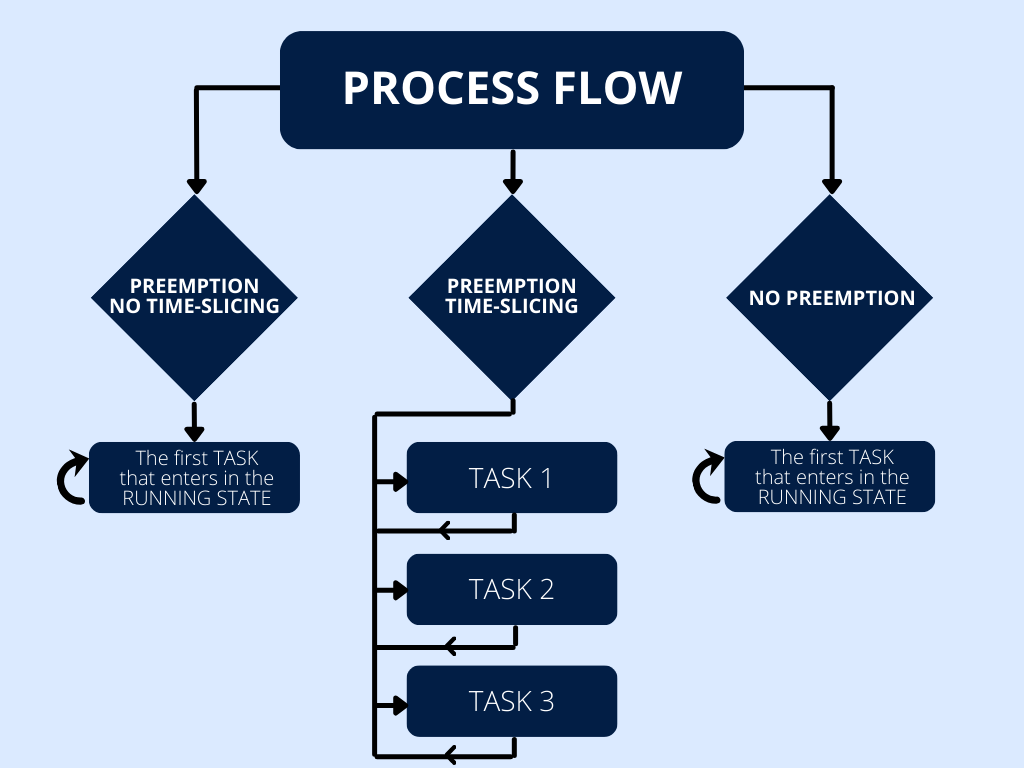
\includegraphics[width=0.5\textwidth]{img/three_tasks_CRUDE.png}
    \caption{Process Flow - main\_three\_tasks\_CRUDE.c}
    \label{fig:Process Flow - CRUDE DELAY}
\end{figure}


\paragraph{Example with DELAY/SLEEP FUNCTION.} 
\label{par: Simple Example with DELAY/SLEEP FUNCTION} 
The \texttt{main\_three\_tasks.c} application is a revised version of the previous one. The unique difference consists in the \textbf{implementation of the delay}. In this case the \textbf{API function} \texttt{vTaskDelayUntil()} offered by \textbf{FreeRTOS} is used to delay the task. This function just moves the task in the \textbf{blocked state}, making room for tasks in the \textbf{ready state}

Considering our demo application, the three tasks \textbf{alternate each other} independently from the \textbf{scheduler configuration}.

\begin{figure}[H]
    \centering
    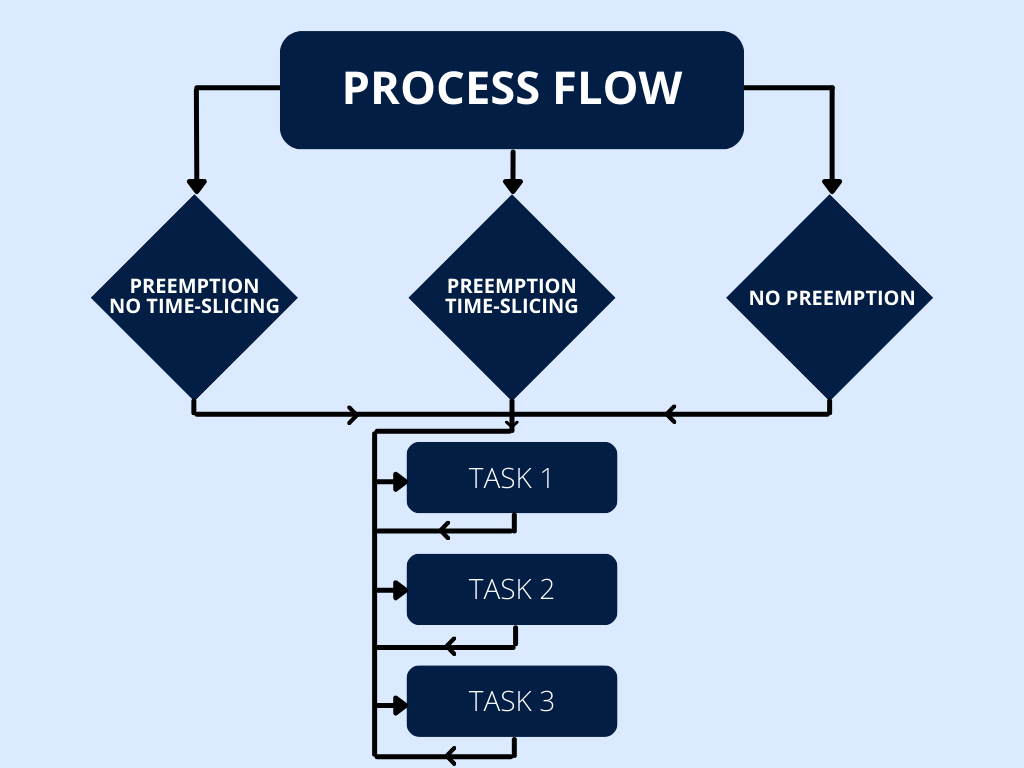
\includegraphics[width=0.5\textwidth]{img/three_tasks.png}
    \caption{Process Flow - main\_three\_tasks.c}
    \label{fig:Process Flow - vTaskDelayUntil}
\end{figure}

\paragraph{Example with Dynamic Priority.} 
\label{par: Simple Example with Dynamic Priority}
The \texttt{main\_priority.c} application is a more advanced example which aims to show how \textbf{FreeRTOS scheduler} works by analysing the behaviour of two tasks where one of them has dynamic priority.
The demo application consists of two tasks:
\begin{itemize}
    \item the \textbf{TASK 2} with lower priority (PRIORITY = 1), which creates the second task \textbf{TASK 1} (at the beginning with PRIORITY = 2), then enters in an infinite loop wherein it prints a message.
    \item the \textbf{TAKS 1} which continously changes its priority, first making it equal to \textbf{TASK 2}'s one, then increasing it again and so on...
\end{itemize}
\textbf{BOTH} the tasks implement a \textbf{CRUDE DELAY} with a for which consumes \textbf{CPU time} (i.e., the tasks are not moved into the waiting list).

The general behaviour of the three tasks changes by modifying the scheduler configurations:
\begin{itemize}
    \item \texttt{configUSE\_PREEMPTION = 1} and \texttt{configUSE\_TIME\_SLICING = 0} $\rightarrow$ the scheduler will be \textbf{preemptive}, \textbf{priority-based} with \textbf{no time slicing} (i.e., ROUND ROBIN DISABLED). In this case, \textbf{TASK 2} creates \textbf{TASK 1} which preempts \textbf{TASK 2} and continues to run.
    \item \texttt{configUSE\_PREEMPTION = 1} and \texttt{configUSE\_TIME\_SLICING = 1} $\rightarrow$ the scheduler will be \textbf{preemptive}, \textbf{priority-based} with \textbf{time slicing enabled} (i.e., ROUND ROBIN-LIKE). 
    In this case, \textbf{TASK 2} creates \textbf{TASK 1} which preempts \textbf{TASK 2}. When \textbf{TASK 1} decreases its priority, the two tasks alternate each other. At a certain point \textbf{TASK 1} increases again its priority continuing to run, and the same cycle will be repeated indefinitely.
    \item \texttt{configUSE\_PREEMPTION = 0} and \texttt{configUSE\_TIME\_SLICING = x} $\rightarrow$ the scheduler will be \textbf{NOT preemptive} and \textbf{priority-based}. 
    In this case, \textbf{TASK 2} creates \textbf{TASK 1} which \textbf{cannot} preempt \textbf{TASK 2} which continues to run indefinitely.
\end{itemize}

\begin{figure}[H]
    \centering
    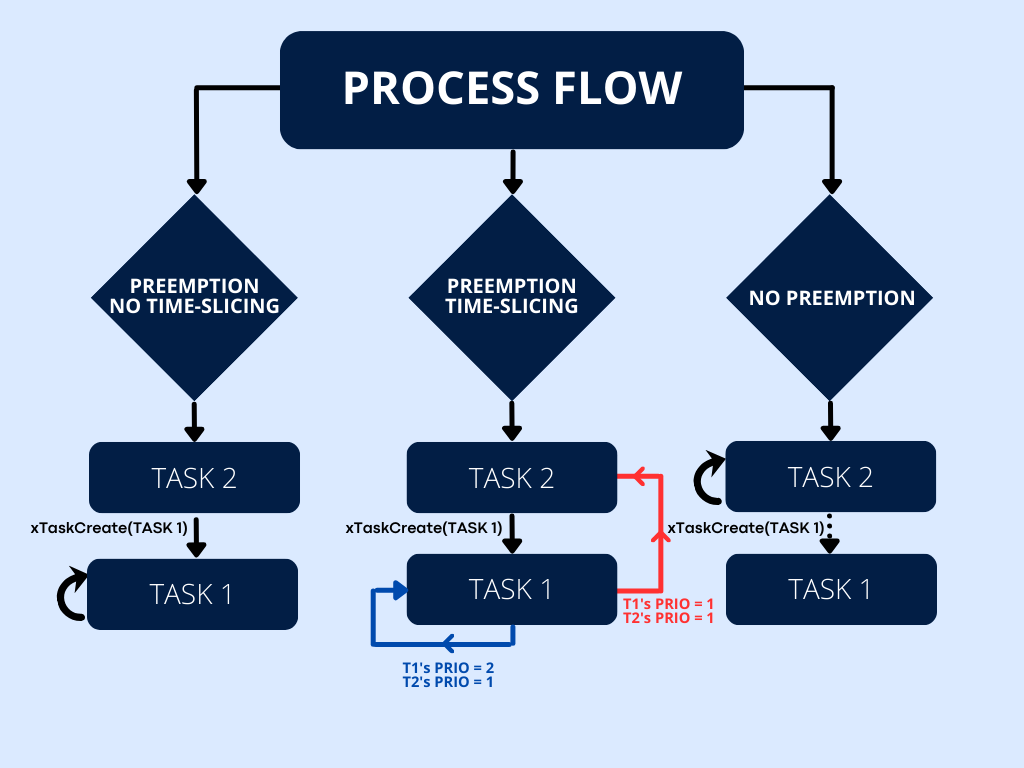
\includegraphics[width=0.5\textwidth]{img/dynamic_priority.png}
    \caption{Process Flow - main\_priority.c}
    \label{fig:Process Flow - Dynamic Priority}
\end{figure}

\subsubsection{Queue and Tasks' Synchronization}
\label{subsubsec: Queue and Tasks' Synchronization}

This subsection provides three different demo applications:
\begin{enumerate}
    \item \texttt{mainCREATE\_SIMPLE\_DEMO = 4} selects the \texttt{main\_queue.c} demo application.
    \item \texttt{mainCREATE\_SIMPLE\_DEMO = 5} selects the \texttt{main\_semaphore.c} demo application.
    \item \texttt{mainCREATE\_SIMPLE\_DEMO = 6} selects the \texttt{main\_semaphore2.c} demo application.
\end{enumerate}
Each of them aims to let the reader understanding:
\begin{itemize}
    \item how to use queues for task-to-task communication. 
    \item how use queues and semaphores for tasks'synchronization.
\end{itemize}

\paragraph{Simple Queue Example}. 
\label{par: Simple Queue Example}
This demo application shows the main \textbf{FreeRTOS API} functions for \textbf{Queue Management}. \textbf{Queues} provide \textbf{Task-to-Task} communication mechanism.
The \texttt{main\_queue} creates \textit{four tasks}:
\begin{itemize}
    \item three \textbf{PRODUCERS} which send items in the queue;
    \item one \textbf{CONSUMER} which reads from the queue.
\end{itemize}
The \textbf{CONSUMER} has the highest priority, the three \textbf{PRODUCERS} have the same priority.

When the scheduler starts the \textbf{CONSUMER} task tries to read from the queue which is empty. The \textbf{CONSUMER} task will block for \texttt{100 ms} waiting for data to be available. At this point one of the \textbf{PRODUCERS} will send data to the queue, unblocking the \textbf{CONSUMER} which will read the data from the queue. The \textbf{CONSUMER} task will then block again waiting for data and the cycle will continue. In this way the \textbf{PRODUCERS} will synchronize with the \textbf{CONSUMER} by just leveraging the \textbf{FreeRTOS queue implementation}.

Sometimes if the \texttt{100 ms} elapses while the queue is still empty, the \textbf{CONSUMER} task will print an \textbf{error message}. Moreover, each task contains a \textbf{CRUDE DELAY} implementation for \textbf{demonstration purposes}.
The general behaviour is depicted in the following diagram:

\begin{figure}[H]
    \centering
    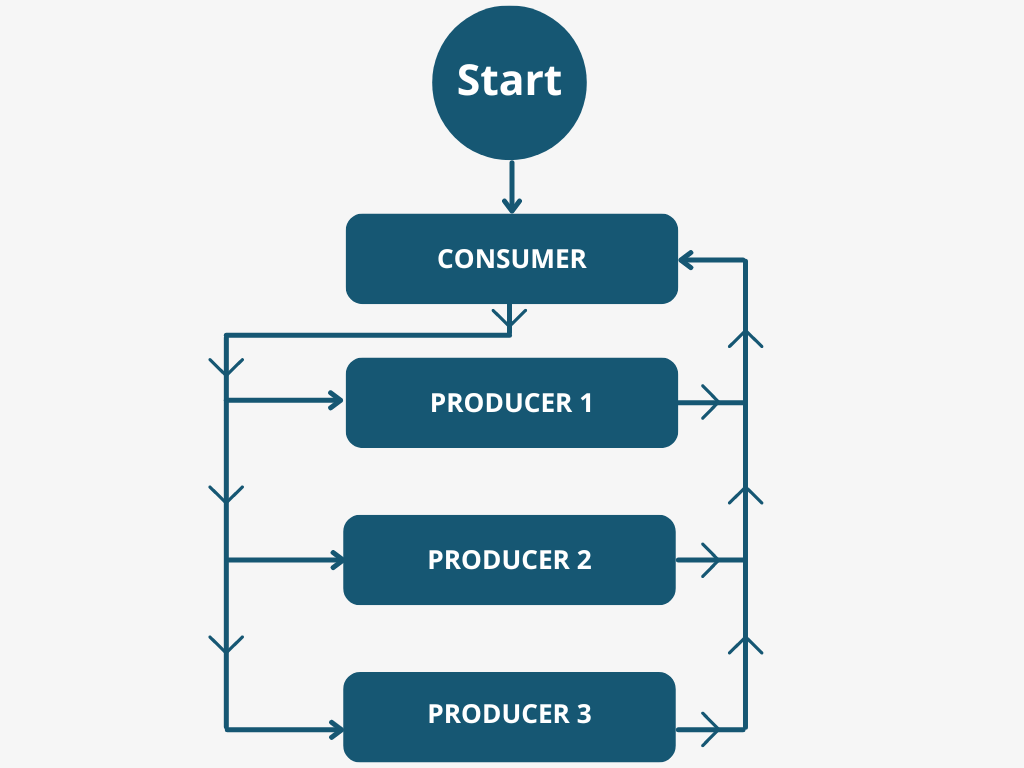
\includegraphics[width=0.5\textwidth]{img/main_queue.png}
    \caption{Precedence Diagram - Queue}
    \label{fig:Precedence Diagram - Queue}
\end{figure}


\paragraph{Queue and Semaphores: Example 1}.
\label{par:Queue and Semaphores 1}
This demo application shows the main \textbf{FreeRTOS} API functions for \textbf{Tasks' Synchronization} using \textbf{semaphores}. \textbf{Semaphores} are objects used to send interrupts for unblocking tasks. This results in tasks synchronization with interrupts.
The \texttt{main\_semaphore} creates the \textbf{queue}, the \textbf{semaphores} and \textbf{four tasks} with the \textbf{SAME priority}:
\begin{itemize}
    \item three \textbf{PRODUCERS} which send items in the queue.
    \item one \textbf{CONSUMER} which reads from the queue.
\end{itemize}
Totally there are two \textbf{binary semaphores}:
\begin{itemize}
    \item one for \textbf{PRODUCERS}.
    \item one for the \textbf{CONSUMER}.
\end{itemize}
At the beginning the main unblocks the \textbf{PRODUCERS}, calling \texttt{xSemaphoreGive(xSemaphoreProducer)} which start to fill the queue. \\ When the queue is full, the \textbf{CONSUMER} can start to read (the \texttt{xSemaphoreGive(xSemaphoreConsumer)} is called). When the \textbf{CONSUMER} reads out all the values in the \textbf{queue}, it unblocks the \textbf{PRODUCERS} and the process will be repeated again.
It's clear that in yhis case the \textbf{priority} fo the tasks is not important, because the sempahores are used to syncronize the tasks. \textbf{Any priority can be used}.
The general behaviour is depicted in the following diagram:

\begin{figure}[H]
    \centering
    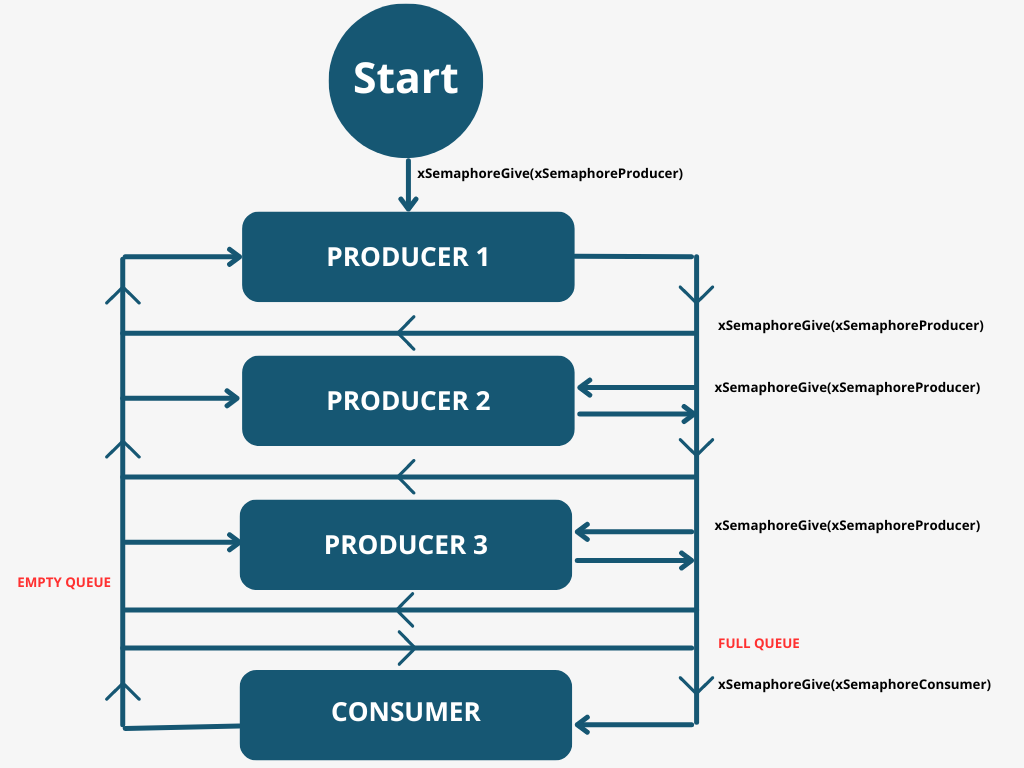
\includegraphics[width=0.5\textwidth]{img/precedence_diagram_semaphore1.png}
    \caption{Precedence Diagram - Semaphores (Example 1)}
    \label{fig:Precedence Diagram - Semaphores (Example 1)}
\end{figure}


\paragraph{Queue and Semaphores: Example 2}.
\label{par:Queue and Semaphores 2}
This demo application is a more advanced example which shows the usage of semaphores for tasks' synchronization.
The \texttt{main\_semaphore2} creates the \textbf{queue}, the \textbf{semaphores} and \textbf{four tasks} with the \textbf{SAME priority}:
\begin{itemize}
    \item three \textbf{PRODUCERS} which send items in the queue;
    \item one \textbf{CONSUMER} which reads from the queue.
\end{itemize}
Totally there are four \textbf{semaphores}:
\begin{itemize}
    \item three \textbf{binary semaphores} for the three \textbf{PRODUCERS};
    \item one \textbf{counting semaphore} for the \textbf{CONSUMER}.
\end{itemize}
Each \textbf{PRODUCER} inserts its value in the queue increasing the value of the counting semaphore of the \textbf{CONSUMER} (i.e, the value of \texttt{xSemaphoreConsumerCounting} represents the number of items currently available in the queue). Then it unblocks the next task as depicted in the following diagram:

\begin{figure}[H]
    \centering
    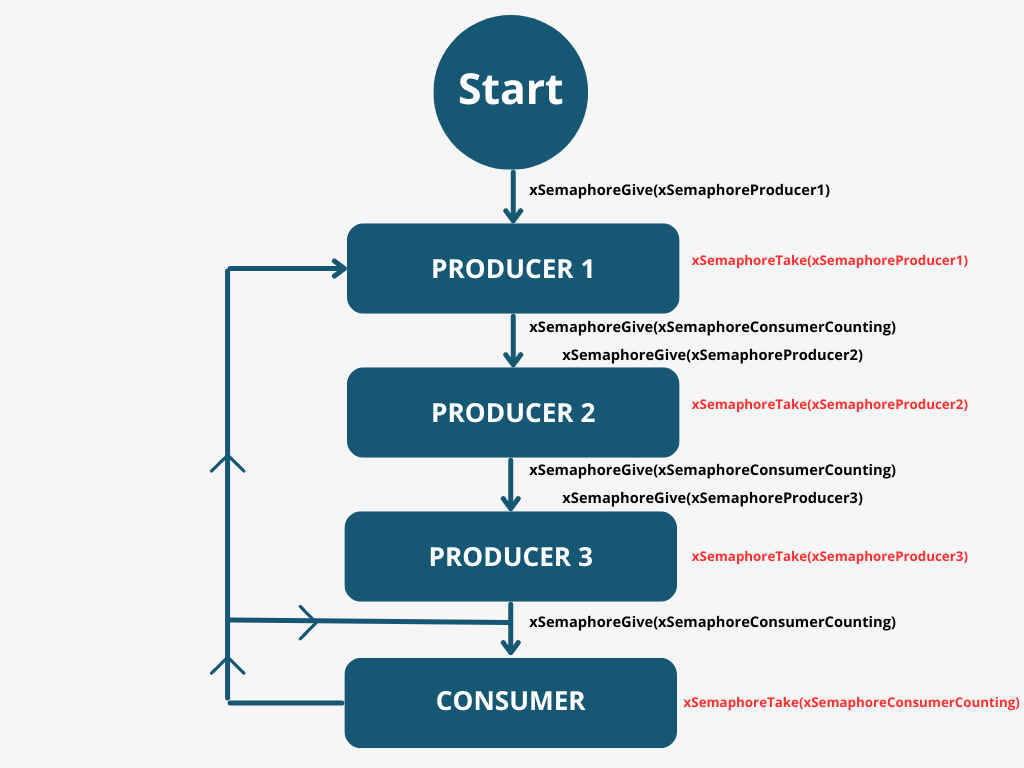
\includegraphics[width=0.5\textwidth]{img/precedence_diagram_semaphore2.png}
    \caption{Precedence Diagram - Semaphores (Example 2)}
    \label{fig:Precedence Diagram - Semaphores (Example 2)}
\end{figure}

Overall, each \textbf{PRODUCER} inserts its value and unblock the next task; then the \textbf{CONSUMER} reads out all the values previously inserted by the \textbf{PRODUCERS} before unblocking the \textbf{first PRODUCER} and the cycle continues indefinitely.
Again here the \textbf{priority} does not change the behaviour of the task.

\section{Memory Management}
\label{sec: Memory Management}
This section introduces the implementation of some heap allocation algorithms. \textbf{FreeRTOS} already provides some implementation for dynamic allocation (\texttt{heap\_x.c}).
This project provides a revised version of \texttt{heap\_4.c} (\texttt{heap\_4\_revised.c}). The standard implementation of \texttt{heap\_4.c} uses by default the \textbf{first-fit} algorithm. The \texttt{heap\_4\_revised.c} version offers the possibility to choose an allocation algorithm among \textbf{first-fit}, \textbf{best-fit} and \textbf{worst-fit} by properly setting the \texttt{configHEAP\_ALLOCATION\_TYPE}'s value in the \texttt{FreeRTOSConfig.h} file.

\subsection{Best-fit}
\label{subsec: Best-Fit}
\paragraph{Best-fit.} The best fit memory allocation strategy allocates the smallest available block that is still large enough to satisfy the requested size.
\begin{lstlisting}[language=C,caption={Custom implementation of Best-Fit algorithm added to heap\_4.c}]
if (configHEAP_ALLOCATION_TYPE == 1)
    configASSERT( heapSUBTRACT_WILL_UNDERFLOW( pxBlock->xBlockSize, xWantedSize ) == 0 );
    /* traverse the whole free block list */
    while( pxBlock->pxNextFreeBlock != heapPROTECT_BLOCK_POINTER( NULL ) )
    {
        /* Check if the current block is a valid option and if another valid block
           was found before and check whether is a best fit */
        if  (   ( pxBlock->xBlockSize >= xWantedSize )
                &&
                (   pxBlockTmp == NULL
                    ||
                    ( ( pxBlock->xBlockSize - xWantedSize ) < ( pxBlockTmp->xBlockSize - xWantedSize ) )
                )
            )
        {
            pxPreviousBlockTmp = pxPreviousBlock;
            pxBlockTmp = pxBlock;
        }
        pxPreviousBlock = pxBlock;
        pxBlock = heapPROTECT_BLOCK_POINTER( pxBlock->pxNextFreeBlock );
        heapVALIDATE_BLOCK_POINTER( pxBlock );
    }
    pxPreviousBlock = pxPreviousBlockTmp;
    pxBlock = pxBlockTmp;
\end{lstlisting}

\subsection{Worst-fit}
\paragraph{Worst-fit.} The worst fit memory allocation strategy allocates the largest available block of memory that can accommodate the requested size.
\begin{lstlisting}[language=C,caption={Custom implementation of Worst-Fit algorithm added to heap\_4.c}]
#elif (configHEAP_ALLOCATION_TYPE == 2)
    configASSERT( heapSUBTRACT_WILL_UNDERFLOW( pxBlock->xBlockSize, xWantedSize ) == 0 );
    /* traverse the whole free block list */
    while( pxBlock->pxNextFreeBlock != heapPROTECT_BLOCK_POINTER( NULL ) )
    {
        /* Check if the current block is a valid option and if another valid block
           was found before and check wheter is a worst fit */
        if  (   ( pxBlock->xBlockSize >= xWantedSize )
                &&
                (   pxBlockTmp == NULL
                    ||
                    ( ( pxBlock->xBlockSize - xWantedSize ) > ( pxBlockTmp->xBlockSize - xWantedSize ) )
                )
            )
        {
            pxPreviousBlockTmp = pxPreviousBlock;
            pxBlockTmp = pxBlock;
        }
        pxPreviousBlock = pxBlock;
        pxBlock = heapPROTECT_BLOCK_POINTER( pxBlock->pxNextFreeBlock );
        heapVALIDATE_BLOCK_POINTER( pxBlock );
    }
    pxPreviousBlock = pxPreviousBlockTmp;
    pxBlock = pxBlockTmp;
\end{lstlisting}

\subsection{First-Fit}
\paragraph{First-Fit.}The first fit memory allocation strategy allocates the first block of memory that is large enough to satisfy the requested size.

\begin{lstlisting}[language=C,caption={Default implementation of First-fit algorithm}]
#else
    while( ( pxBlock->xBlockSize < xWantedSize ) && ( pxBlock->pxNextFreeBlock != heapPROTECT_BLOCK_POINTER( NULL ) ) )
    {
        pxPreviousBlock = pxBlock;
        pxBlock = heapPROTECT_BLOCK_POINTER( pxBlock->pxNextFreeBlock );
        heapVALIDATE_BLOCK_POINTER( pxBlock );
    }
#endif
\end{lstlisting}


\section{Performance Evaluation}
\label{sec: Performance Evaluation}
This project provides a \textbf{simple demo application} for evaluating the behaviour of the \textbf{allocation algorithms} previously introduced.
The demo application can be selected by setting the \texttt{mainCREATE\_SIMPLE\_DEMO} value to \texttt{7} in the \texttt{main.c} file. 


\subsection{Demo Application}
\label{subsec: Mem Mang Demo App}
The \textbf{main} function performs the following steps:
\begin{multicols}{2} % Inizia l'ambiente a due colonne
\begin{enumerate}
    \item \textbf{Allocates 1000 bytes}
    \item \textbf{Allocates 1000 bytes}
    \item \textbf{Allocates 1500 bytes}
    \item \textbf{Allocates 100 bytes}
    \item \textbf{Allocates 100 bytes}
    \item \textbf{Allocates 100 bytes}
    \item \textbf{Allocates 100 bytes}
    \item \textbf{De-allocates 1000 bytes (second block)}
    \item \textbf{De-allocates 100 bytes (fourth block)}
    \item \textbf{De-allocates 100 bytes (fifth block)}
    \item \textbf{De-allocates 100 bytes (sixth block)}
    \item \textbf{Allocates 300 bytes}
    \item \textbf{Allocates 1000 bytes}
    \item \textbf{Creates a task (TASK 1)}
\end{enumerate}
\end{multicols}

After each operation, \textbf{the free heap space} and \textbf{the minimum ever free heap space} are recorded. If an allocation fails, the system prints an error message using the \texttt{vApplicationMallocFailedHook} function in `main.c`.

\subsection{Evaluation}
\label{subsec: Evaluation}
For this test, the heap size \texttt{(configTOTAL\_HEAP\_SIZE)} in the \texttt{FreeRTOSConfig.h} file is set to \textbf{4 kB}.

\subsubsection{First-Fit Algorithm}
When the default implementation is selected (i.e., \textbf{First-Fit}), the allocation fails before the last block of \textbf{1000 bytes} is allocated. The output obtained is shown in Table \ref{tab:firstfit}.

\begin{longtable}{|l|c|c|}
    \hline
    \textbf{Message} & \textbf{Free Heap (B)} & \textbf{Minimum Ever Free Heap (B)} \\
    \hline
    1. Before allocating memory blocks & 0 & 0 \\
    2. After allocated 1000 bytes & 3072 & 3072 \\
    3. After allocated 1000 bytes & 2064 & 2064 \\
    4. After allocated 1500 bytes & 552 & 552 \\
    5. After allocated 100 bytes & 440 & 440 \\
    6. After allocated 100 bytes & 328 & 328 \\
    7. After allocated 100 bytes & 216 & 216 \\
    8. After allocated 100 bytes & 104 & 104 \\
    9. After deallocated the second block (1000 bytes) & 1112 & 104 \\
    10. After deallocated the fourth block (100 bytes) & 1224 & 104 \\
    11. After deallocated the fifth block (100 bytes) & 1336 & 104 \\
    12. After deallocated the sixth block (100 bytes) & 1448 & 104 \\
    13. After allocated 300 bytes & 1136 & 104 \\
    \hline
    \textbf{Malloc failed..} & & \\
    \hline
    \caption{Worst-Fit Allocation Algorithm Results}
    \label{tab:firstfit}
\end{longtable}

The \textbf{heap configuration} at \textbf{step 13} (i.e., before the failure) is the following:

\begin{figure}[H]
    \centering
    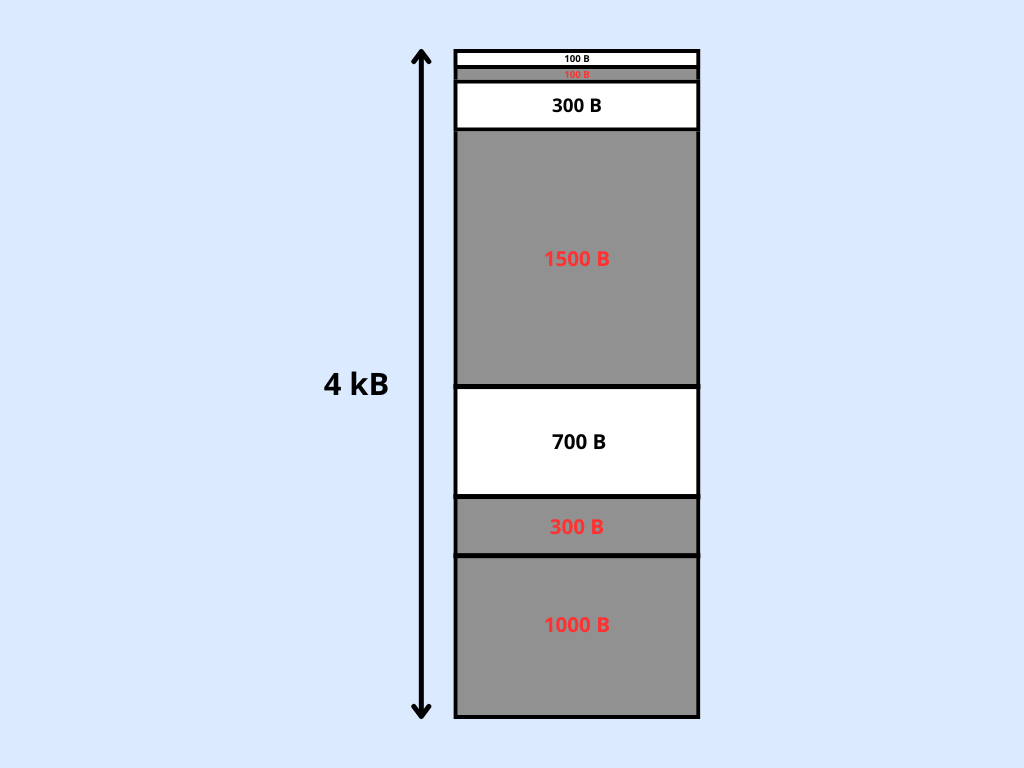
\includegraphics[width=0.5\textwidth]{img/first-worst.png}
    \caption{Heap Configuration - First-Fit}
    \label{fig:Heap Configuration - First-Fit}
\end{figure}

\newpage
\subsubsection{Best-Fit Algorithm}
When the Best-Fit algorithm is used, the system fails to allocate memory for creating the task at step 14 because there is insufficient space. The output obtained is shown in Table \ref{tab:bestfit}.
\begin{longtable}{|l|c|c|}
    \hline
    \textbf{Message} & \textbf{Free Heap (B)} & \textbf{Minimum Ever Free Heap (B)} \\
    \hline
    1. Before allocating memory blocks & 0 & 0 \\
    2. After allocated 1000 bytes & 3072 & 3072 \\
    3. After allocated 1000 bytes & 2064 & 2064 \\
    4. After allocated 1500 bytes & 552 & 552 \\
    5. After allocated 100 bytes & 440 & 440 \\
    6. After allocated 100 bytes & 328 & 328 \\
    7. After allocated 100 bytes & 216 & 216 \\
    8. After allocated 100 bytes & 104 & 104 \\
    9. After deallocated the second block (1000 bytes) & 1112 & 104 \\
    10. After deallocated the fourth block (100 bytes) & 1224 & 104 \\
    11. After deallocated the fifth block (100 bytes) & 1336 & 104 \\
    12. After deallocated the sixth block (100 bytes) & 1448 & 104 \\
    13. After allocated 300 bytes & 1136 & 104 \\
    14. After allocated 1000 bytes & 128 & 104 \\
    \hline
    \textbf{Malloc failed...} & & \\
    \hline
    \caption{Best-Fit Allocation Algorithm Results}
    \label{tab:bestfit}
\end{longtable}

At step 14, the allocation fails because there is not enough space to create the \textbf{TCB} (\textbf{Task Control Block}).
The \textbf{heap configuration} at \textbf{step 14} (i.e., before the failure) is the following:

\begin{figure}[H]
    \centering
    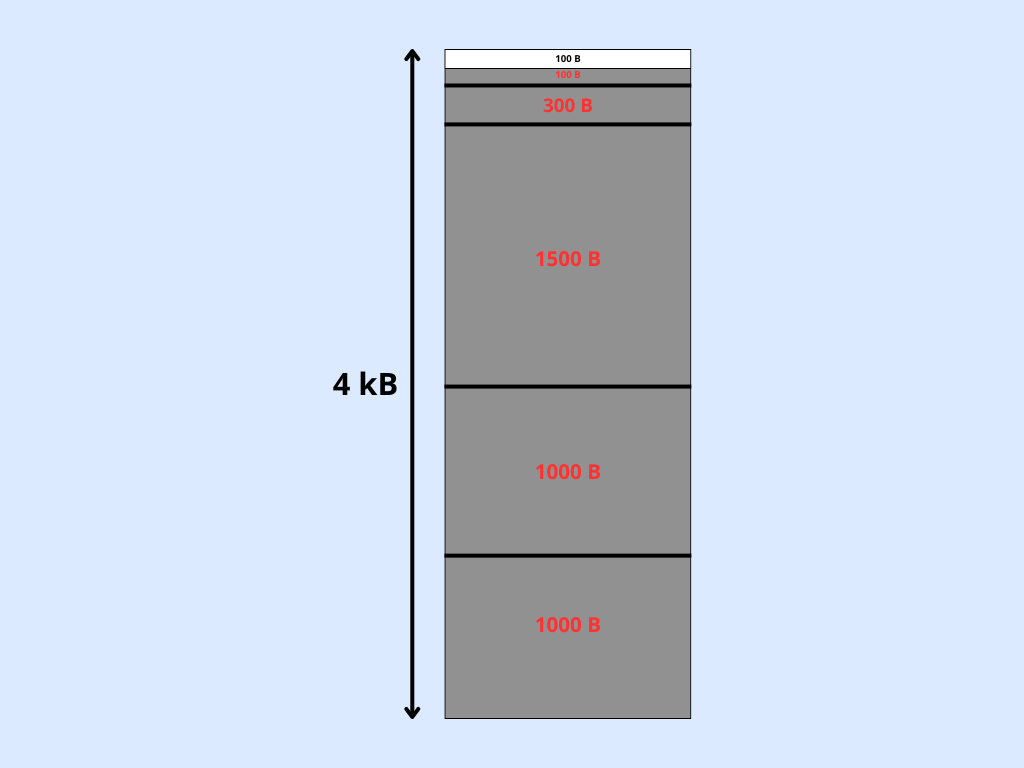
\includegraphics[width=0.5\textwidth]{img/best.png}
    \caption{Heap Configuration - Best-Fit}
    \label{fig:Heap Configuration - Best-Fit}
\end{figure}

\subsubsection{Worst-Fit Algorithm}
The output is the same obtained with \textbf{First-Fit} algorithm in Table \ref{tab:firstfit} (i.e., in this specific example the two algorithms behave in the same way). Obviously also the heap configuration before the failure is the same \ref{fig:Heap Configuration - First-Fit}.



\newpage
\section{Conclusions}
Our project aims to show the use of \textbf{FreeRTOS} on \textbf{Qemu} through tutorials, exercises and modifying some solutions of the operating system. 
Some demo applications were developed to provide a comprehensive overview on FreeRTOS' \textbf{task management}, \textbf{queue and semaphore's usage} for \textbf{task-to-task communication and tasks' synchronization}. Next, new implementations of heap allocation algorithms were implemented by revising the \texttt{heap\_4.c} file provided with the FreeRTOS distribution. Particularly, the \textbf{Best-Fit} and \textbf{Worst-Fit} algorithms are added to the \textbf{First-Fit} one, which is the default choice. Finally, a demo application was developed to evaluate the newly implemented solution. Overall, developing this project helps us to gain the main skills in \textbf{FreeRTOS programming}, to better understand \textbf{embedded systems} and \textbf{real time operating systems}. 

\section{Statement Of Work}

The work of each member of the group is summarised below.

\begin{table}[h!]
    \centering
    \begin{tabular}{|c|l|}
        \hline
        \textbf{Member} & \textbf{Work Done} \\ \hline
        Rachid Youssef Grib & 
        \begin{tabular}[c]{@{}l@{}}
            Memory Management, Queue and Tasks Synchronization
        \end{tabular} \\ \hline
        Giuseppe Famà & 
        \begin{tabular}[c]{@{}l@{}}
           Installation, Queue and Tasks Synchronization
        \end{tabular} \\ \hline
        Vincenzo Longo & 
        \begin{tabular}[c]{@{}l@{}}
            Installation, Tasks Management
        \end{tabular} \\ \hline
    \end{tabular}
\end{table}

\noindent The job was done in \textbf{presence}, \textbf{all the participants actively participated} to this project.

\end{document}
